% !TeX root = ../main.tex
\chapter{实验一:用户任意桌面点击行为规律}
\label{cha:exp1}
虽然相关文献已经表明用户能够将双手盲打的肌肉记忆迁移到不同的应用场景,例如大尺寸触摸屏、单手输入等等。然而,由于我们的交互界面并非触摸屏,而是一般的桌面,由于材质不同,用户输入时的触感也有一定差异。因此我们通过此实验进一步探究在普通桌面上用户双手输入的习惯和行为规律。


\section{被试}
在桌面上十指输入的实验中,我们一共招募了X名被试(男性X人,女性X人),平均年龄为X岁(标准差=X)。所有人都具有在物理键盘上熟练打字的使用习惯。此外,在正式实验开始前,我们首先使用Wobbrock编写的TextTest软件\cite{texttest}\cite{wobbrock2006analyzing}测试了他们在实体键盘上的打字速度和准确度。经过测试,被试们的输入速度为X单词每分钟,无纠正情况的错误率为X\%。每位被试获得50元作为实验报酬。

\section{实验装置和实验平台}
\begin{figure}[h] % use float package if you want it here
    \centering
    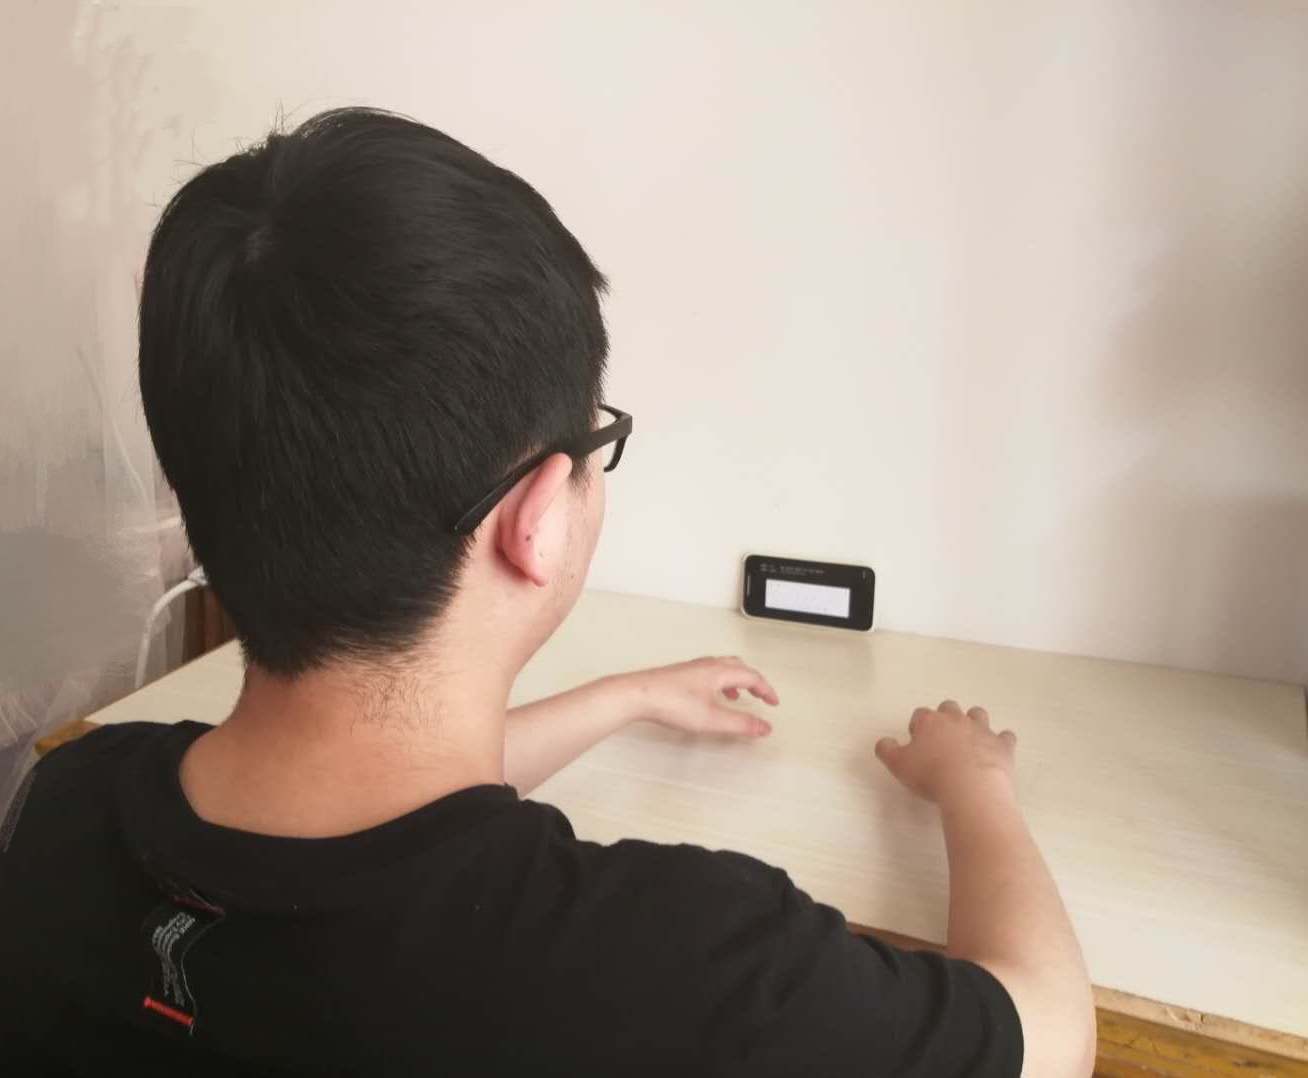
\includegraphics[height=6cm]{exp.jpeg}
    \caption{用户在桌面上输入的场景}
    \label{fig:exp}
\end{figure}
我们使用Swift和Objective-C在iPhone 11上开发了APP作为实验平台,XCode为开发环境。其中第~\ref{cha:sensing}~章已经对于手机如何获取并处理传感信息做了具体介绍,我们程序记录下了每次点击的坐标位置和相应时间戳。手机不仅用来接收传感信号,同时也向用户展示了实验平台。手机的屏幕尺寸为6.1英寸。在使用时,用户的双手距离手机约15-30厘米。为了充分利用手机的视场角,用户两手中心和手机的前置摄像头基本处于同一竖直线上。这样摄像头能够较为完整捕捉到手部的运动信息。图~\ref{fig:exp}~展示了用户进行实验时的状态。为了避免外界声音的干扰,实验在较为安静的室内空间进行。

图~\ref{fig:platform0}~展示了实验时手机上的界面。界面上显示了当前的实验进度以及用户要输入的目标句子。另外,为了防止用户遗忘物理键盘布局,我们在界面下方放置了一个标准的QWERTY键盘作为参考。

\begin{figure}[h] % use float package if you want it here
    \centering
    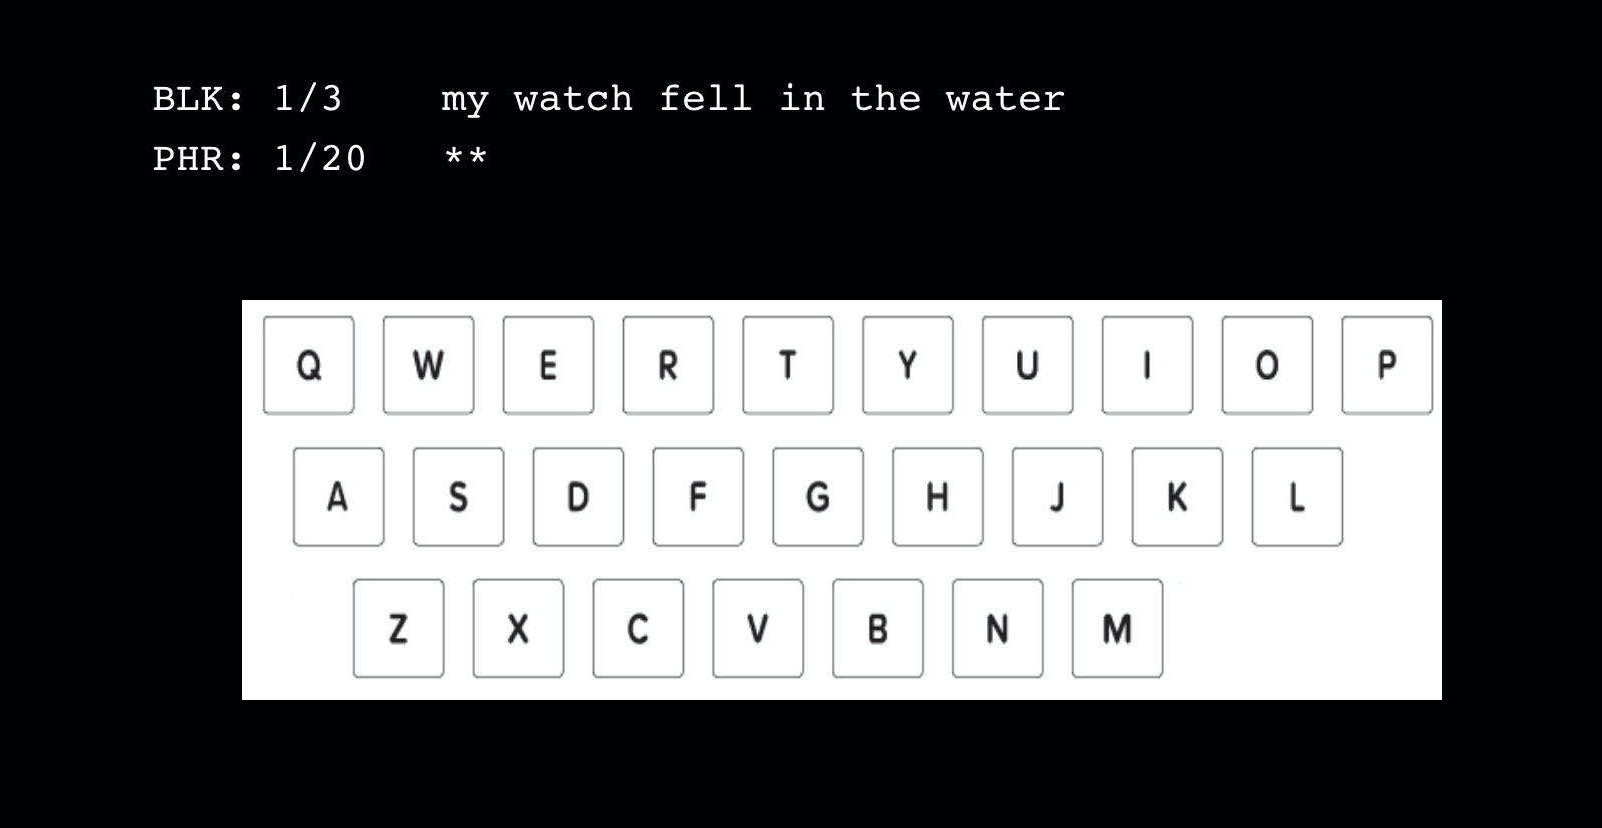
\includegraphics[height=5cm]{platform0.jpeg}
    \caption{iPhone11上实验平台界面}
    \label{fig:platform0}
\end{figure}

和前人工作类似\cite{flatglass2011findlater}\cite{2017blindtype},在打字的过程中,如图~\ref{fig:platform0}~所示,我们提供星号作为视觉反馈。这是为了尽可能减小不同输入纠错算法对用户本身的输入行为造成影响。另外,基于第~\ref{cha:sensing}~章的点击识别算法,每次识别到用户的点击,星号的数目会相应增加一个。


\section{实验设计及流程}
每位用户一共需要输入60句话,分为4部分,我们称为输入块。每个输入块一共有15句话,其中有13句是从Mackenzie提出的短语库\cite{mackenzie2003phrase}中随机选择的,另外两句均是相同的全字母句“The quick brown fox jumps over the lazy dog”和“The five boxing wizards jump quickly”,保证了每个用户都能够输入字母表中所有字母。

用户坐在手机前进行整个实验流程。在实验开始前,我们会简要介绍实验的目的并且指示用户尽可能快而准确地输入。用户将有3分钟的时间用于熟练实验平台。每当用户输入完一句话后,右手进行右移进入下一个句子。为了防止手部疲劳,每输入完一句话用户可以将手放在桌面上休息,每输入完一个输入块用户会需要强制休息2分钟。此外,当用户察觉到自己输入错误时,可以左手左划清空本句的数据并重新输入。实验结束后,我们会搜集用户的基本信息,并针对输入体验、速度、使用习惯等问题以及相关建议对用户进行一个简要的访谈。

\section{实验结果}
从XX名用户的数据中,我们一共收集了XX个落点。为了减小偶然误差的影响,对于每个按键,我们移除了各方向超过3倍标准差的落点,一共有XX个,占所有落点XX的比例。

\subsection{输入速度}
我们输入速度的计算使用MacKenzie提出的公式\cite{speedcalc},单位是WPM,即单词每分钟。

\begin{equation}
    \label{calcspeed}
    WPM = \frac{|L|-1}{T} \times 60 \times \frac{1}{5}
\end{equation}

其中,$|L|$是输入的某段文本的长度,在我们的计算中即从一句话第一个字符到最后一个字符所有字符数,$T$是输入这句话所用的总时间,单位为秒。

输入的平均速度为43(SD = XX)WPM,速度范围为XX WPM到XX WPM,该速度要慢于在物理键盘上的速度。从图~\ref{fig:speed0}~中可以看出,输入速度随着输入块单调递增,在最后一个输入块能够超过45WPM。平均速度快于同样有星号反馈情况下在触摸屏上十指盲打\%\cite{flatglass2011findlater},慢于物理键盘上的平均输入速度。速度的趋势说明用户能够逐渐适应并熟练掌握在桌面上输入的方式。F检验证明输入块对于输入速度有显著的影响(F=XX, p=XX)。
\begin{figure}[h] % use float package if you want it here
    \centering
    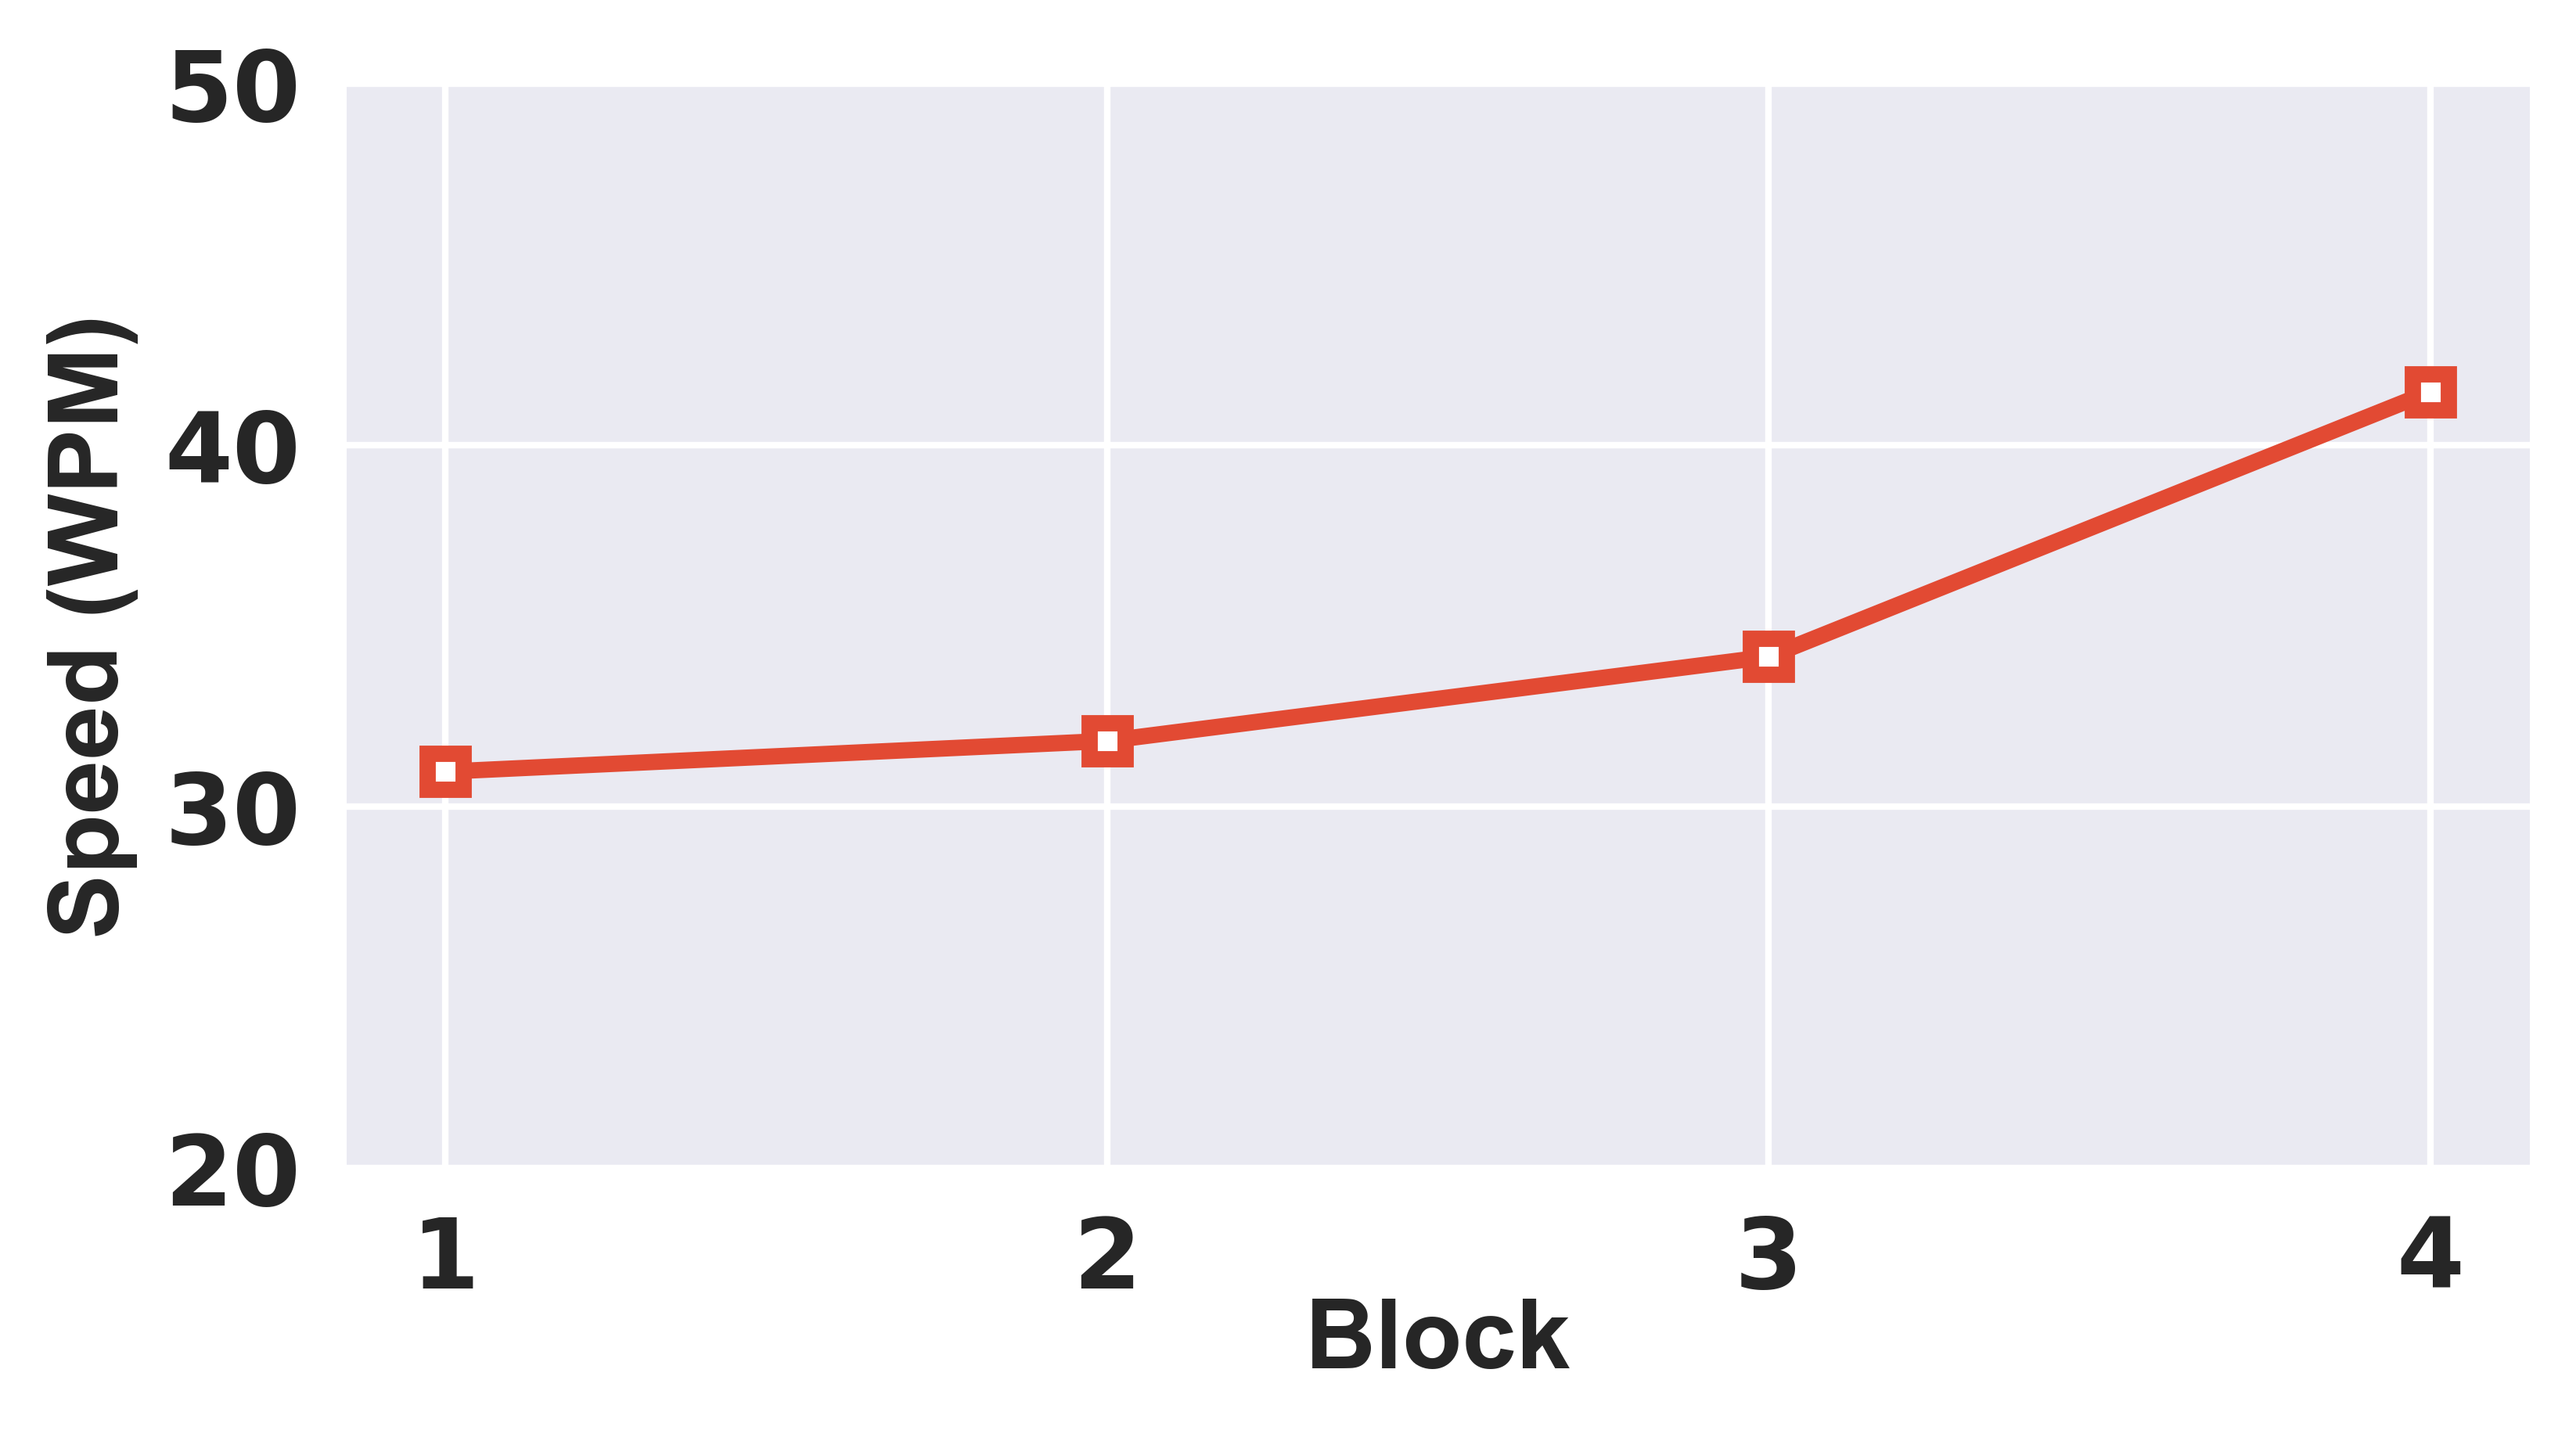
\includegraphics[height=6cm]{speed0.png}
    \caption{实验时每个输入块的平均输入速度}
    \label{fig:speed0}
\end{figure}

\subsection{落点分布}
考虑到不同用户落点分布的绝对位置有一定偏差,我们将所有人F键和J键的中心点平移到了同一位置进行进一步分析\cite{flatglass2011findlater}\cite{palmboard2020}\cite{2018shitoast}。图~\ref{fig:points}~展示了所有用户落点集中后的分布图,可以看出每个按键呈聚集的趋势,但是相邻的按键,尤其是同一行的按键有一定的重合。

\begin{figure}[h] % use float package if you want it here
    \centering
    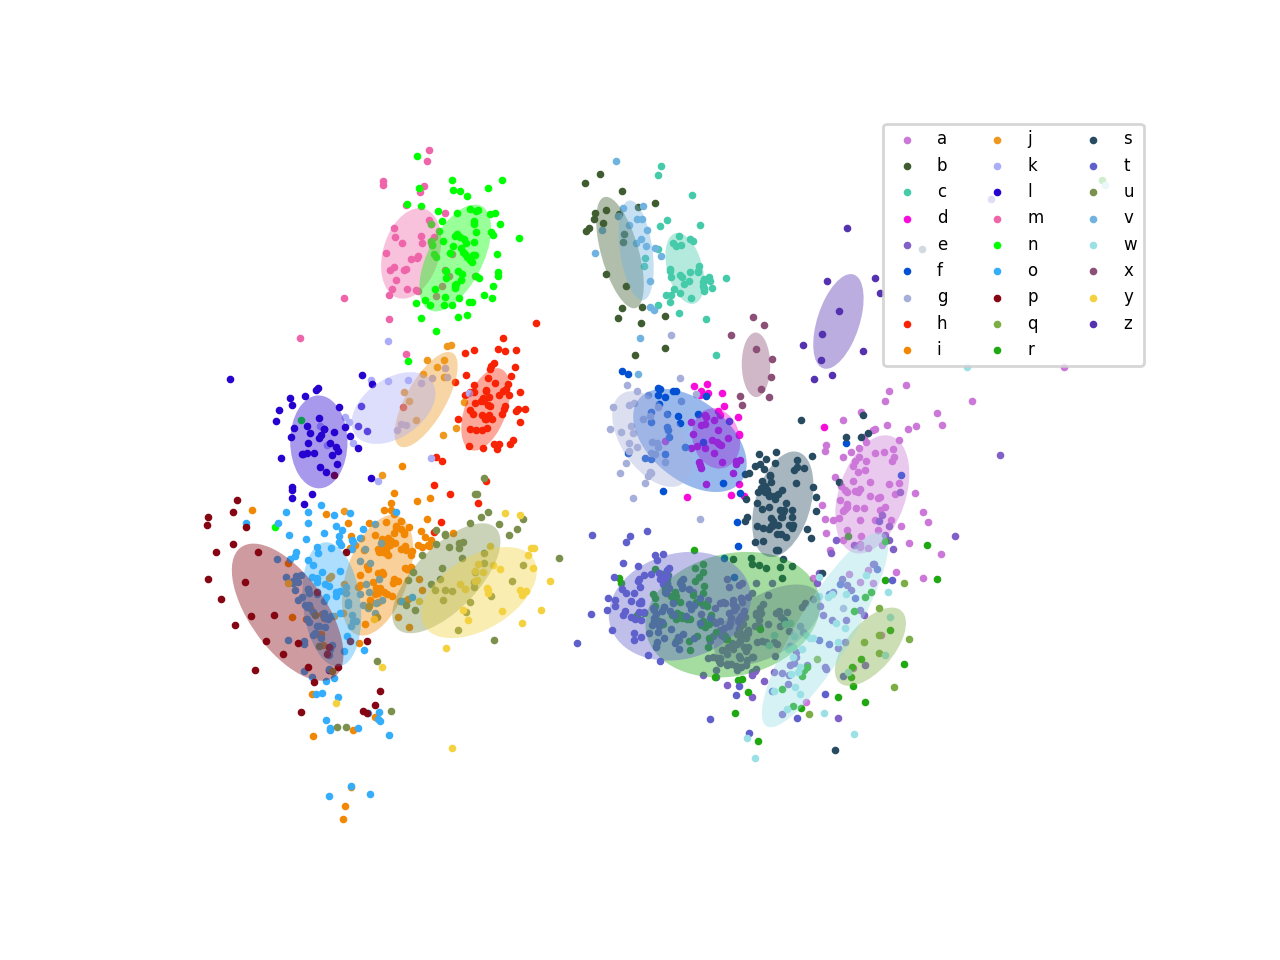
\includegraphics[width=13cm]{touchpoints.png}
    \caption{所有用户的落点分布图,使用颜色区分按键}
    \label{fig:points}
\end{figure}

表~\ref{tab:sd}~展示了字母键和空格键在单人情况下和合并情况下的在横轴和纵轴的标准差。其中平均而言,横轴标准差总是大于纵轴,说明被试相对而言更容易控制纵向的点击,因为横向同一行的按键更多,可能更难控制。然而,底部行(z,x按键所在行)在纵轴上的标准差更大,和文献中结果类似\cite{flatglass2011findlater}。此外,合并后的标准差要大于每个人单独计算的值,说明不同用户的输入控制能力存在一定差异,可能与平时键盘的使用习惯以及手指大小等因素有关。另外,无论是在单人还是所有人的情况下,空格键在两个方向上的标准差均远大于普通字母键,说明在无键盘的情况下,用户心理键盘模型中,空格键仍然和物理键盘上一样占据较大区域。

\begin{table}[htb]
    \centering
    \begin{minipage}[t]{0.7\linewidth} % 如果想在表格中使用脚注,minipage是个不错的办法
    \caption[实验一标准差]{单个人和所有人落点合并在一起的字母键和空格键在X和Y方向的标准差的平均值,括号中为不同人的标准差,其中第二行无标准差}
    \label{tab:sd}
      \centering
      \begin{tabularx}{0.7\linewidth}{c c c}
        \toprule[1.5pt]
        坐标轴 & X & Y\\\midrule[1pt]
        字母键(单人) & 1.1(1.1)& 1.1(1.1)\\
        空格键(单人) & &\\
        字母键(所有人) & & \\
        字母键(所有人) & &\\
        \bottomrule[1.5pt]
      \end{tabularx}
    \end{minipage}
  \end{table}

\subsection{键盘拟合}
使用BlindType\cite{2017blindtype}提出的公式~(\ref{equ:fitkeyboard})对用户点击进行键盘拟合。
\begin{equation}
  \label{equ:fitkeyboard}
  \begin{aligned}
  \textbf{x} &= s_{x} \times \textbf{X} + o_{x} \\
  \textbf{y} &= s_{y} \times \textbf{Y} + o_{y}
  \end{aligned}
\end{equation}

其中$\textbf{x}$和$\textbf{y}$为用户所有点击横纵坐标分别构成的向量,$\textbf{X}$和$\textbf{Y}$为$\textbf{x}$和$\textbf{y}$对应点击的按键在标准物理键盘上的横纵坐标。在两个方向分别进行线性回归,因此$s_{x}$和$s_{y}$表示拟合出的按键在两个方向上的长度,$o_{x}$和$o_{y}$为所拟合出键盘的偏移。表~\ref{tab:fitkeyboard}~中列出了拟合的全键盘按键大小及偏移。可以看到,因为可供用户输入的区域较大,拟合出的按键的尺寸也远大于物理键盘,并且纵轴长于横轴。图~\ref{fig:fitkeyboard}~展示了落点坐标轴的位置和方向,原点处是前置摄像头。根据拟合出的键盘偏移,图中展示了拟合后的键盘大致位置,和用户进行实验时双手放置位置一致。在两个方向上的$R^{2}$都超过了0.85,说明键盘拟合效果较好。

\begin{figure}[h] % use float package if you want it here
  \centering
  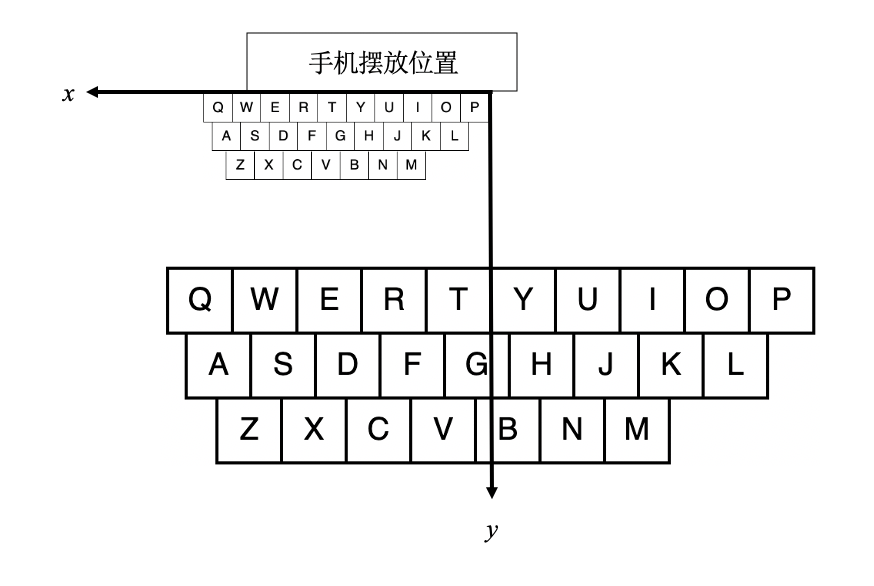
\includegraphics[width=10cm]{fit-keyboard.png}
  \caption{用户位置处的俯视图,较小键盘为拟合前的键盘位置,较大键盘显示了拟合后的位置和大小,实际比例可能有一定误差}
  \label{fig:fitkeyboard}
\end{figure}

\begin{table}[htb]
  \centering
  \begin{minipage}[t]{0.55\linewidth} % 如果想在表格中使用脚注,minipage是个不错的办法
  \caption[拟合出的键盘参数]{拟合出的键盘大小和偏移,括号中为标准差}
  \label{tab:fitkeyboard}
    \centering
    \begin{tabularx}{\linewidth}{cccc}
      \toprule[1.5pt]
      %  & \multicolumn{2}{c}{总体}&\multicolumn{2}{c}{左手} &  \multicolumn{2}{c}{右手} \\\midrule[1pt]
      & 按键大小(cm) & 键盘偏移(cm) & $R^{2}$ \\\midrule[1pt]
      X & 2.67 (0.24) & -13.17 (1.80) & 0.96 \\
      Y & 3.35 (0.38) & 20.24 (1.15) & 0.85\\
      \bottomrule[1.5pt]
    \end{tabularx}
  \end{minipage}
\end{table}

%spread of size
%两手之间的间距

\subsection{键盘落点分布}
图~\ref{fig:keyboard-curve}~展示了所有被试落点合并后的按键中心位置。从按键中心的分布情况可以看出,26个字母的相对位置仍然符合QWERTY布局。但是,不同于标准的物理键盘,落点分布呈现一定的弧形,和在触摸屏上十指盲打结果类似\cite{flatglass2011findlater}\cite{2018shitoast}。使用贝塞尔曲线分别拟合左右手每一行的按键中心如图\ref{fig:keyboard-curve}。

我们计算了最左到最右,最上到最下中心点的距离平均值,分别为22.8cm和7.97cm,可见落点分布范围较大,与拟合出的按键较大结果相一致。左右两只手的中间有一定间隔,说明用户在桌面上进行十指盲打时倾向于将两手分开并保持一定的距离,和在触摸屏上类似\cite{flatglass2011findlater}。
\begin{figure}[ht]
  \centering
  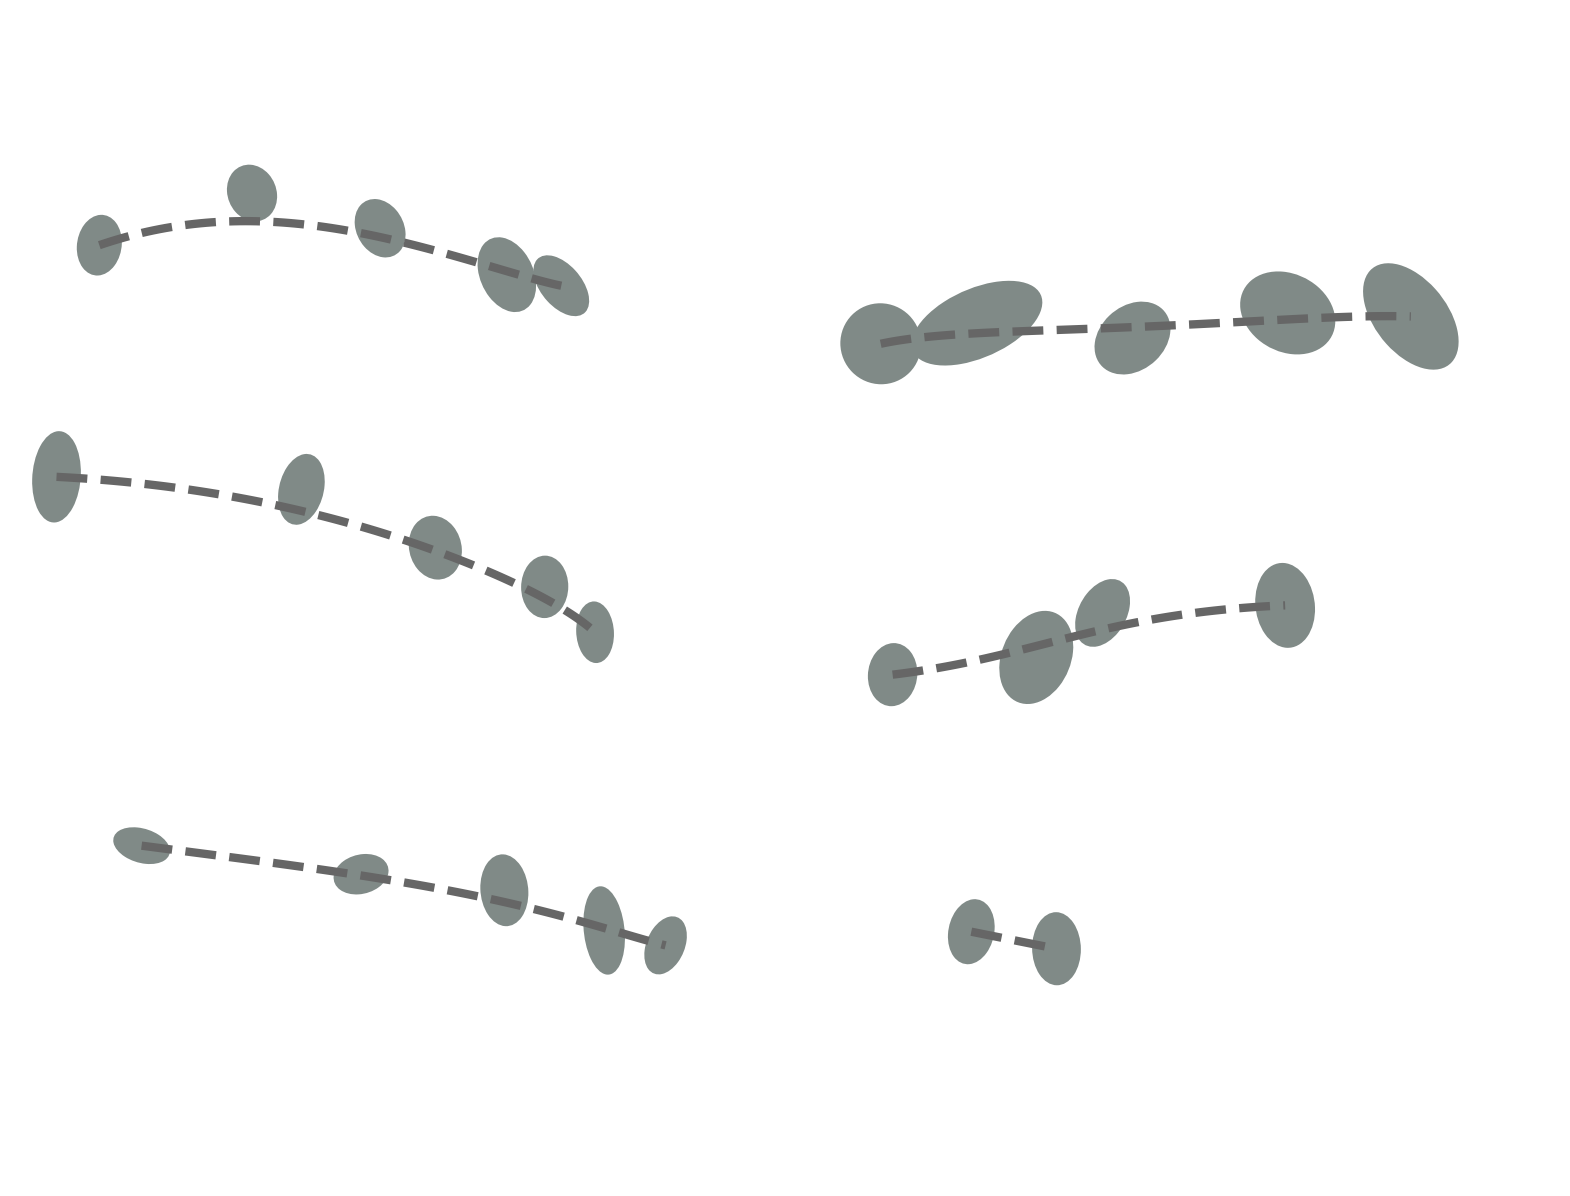
\includegraphics[height=6cm]{curve.png}
  \caption{使用贝塞尔曲线拟合的按键中心点,椭圆为一标准差}
  \label{fig:keyboard-curve}
\end{figure}

\subsection{输入行为}
在一般的触摸屏上例如iPad上十指输入时,因为误触的问题,用户在不输入时将双手放下休息。即使在没有误触时,因为心理因素,有的用户仍然习惯于不放下手\cite{palmboard2020}。在我们的实验中,我们允许并鼓励用户在输入完一个句子后将手放在桌面上休息。经过观察和访谈,我们发现用户愿意将双手放于桌面,并且用户称此行为能够减轻疲劳。

\section{本章总结}
本章通过用户实验,采集了用户在桌面上进行双手盲打的输入数据。我们分析了输入速度、按键大小、落点分布、输入行为等一系列特征,并对比了前人在触摸屏上类似实验。相比而言,我们的输入区域更大,因此拟合的按键也更大,并且能够较好支持用户双手放下休息的行为。